\documentclass[twoside, 12pt]{article}

\usepackage[sc]{mathpazo} % Use the Palatino font
\usepackage[T1]{fontenc} % Use 8-bit encoding that has 256 glyphs
\linespread{1.5} % Line spacing - Palatino needs more space between lines

%\usepackage[twoside,width=16cm,height=24cm,left=3cm]{geometry}
\usepackage[hmarginratio=1:1,top=20mm,width=20cm,height=23.7cm,columnsep=15pt]{geometry} % Document margins
\usepackage{multicol} % Used for the two-column layout of the document
\usepackage[hang, small,labelfont=bf,up,textfont=it,up]{caption} % Custom captions under/above floats in tables or figures
\usepackage{booktabs} % Horizontal rules in tables
\usepackage{float} % Required for tables and figures in the multi-column environment - they need to be placed in specific locations with the [H] (e.g. \begin{table}[H])
\usepackage{hyperref} % For hyperlinks in the PDF

%----------- Agregados para el caso de ustedes -------------------------------
\usepackage[spanish]{babel}% idioma castellano
\usepackage[utf8]{inputenc}% esto es para poder poner los tildes directamente. Puede que cambie de versión a versión de sistema operativos (más información en http://www.aq.upm.es/Departamentos/Fisica/agmartin/webpublico/latex/FAQ-CervanTeX/FAQ-CervanTeX-6.html )
\usepackage{graphicx} % para insertar figuras
\usepackage{subfigure} % para insertar figuras dentro de figuras
\usepackage{times} % plataforma
\usepackage{amsmath} % --para ecuaciones y algunos símbolos 
\usepackage{wrapfig,lipsum}
\usepackage{listings}
\usepackage{color}

\definecolor{dkgreen}{rgb}{0,0.6,0}
\definecolor{gray}{rgb}{0.5,0.5,0.5}
\definecolor{mauve}{rgb}{0.58,0,0.82}

\lstset{frame=tb,
	language=C++,
	aboveskip=3mm,
	belowskip=3mm,
	showstringspaces=false,
	columns=flexible,
	basicstyle={\small\ttfamily},
	numbers=none,
	numberstyle=\tiny\color{gray},
	keywordstyle=\color{blue},
	commentstyle=\color{dkgreen},
	stringstyle=\color{mauve},
	breaklines=true,
	breakatwhitespace=true,
	tabsize=3
}
% ---------------------- -----------------------------------------------------

\usepackage{lettrine} % The lettrine is the first enlarged letter at the beginning of the text
\usepackage{paralist} % Used for the compactitem environment which makes bullet points with less space between them
\usepackage[T1]{fontenc}					%para poder usar tildes sin problemas

\usepackage{mathrsfs}
% Abreviaturas
%\newcommand\RR{\mathbb{R}}

\providecommand{\dpart}[2]{\frac{\partial#1}{\partial#2}}

\graphicspath{{Imagenes/}}

\begin{document}
	
\begin{center}
	{\fontsize{20pt}{10pt}\textbf{Choque unidimensional bajo potencial de Pauli}}
\end{center}

\section{Implementación de Pauli}

\subsection{Características generales}

El potencial de Pauli, debido a su dependencia en el momento, no es candidato para heredar las propiedades de un potencial \texttt{ShortRange} como Morse o Lennard-Jones

\[ V_{P}(q,p) = D\sum_{i<j} e^{-\frac{1}{2}s_{ij}^2} \qquad \text{;} \qquad s_{ij}^2 = \frac{|\mathbf{p}_i - \mathbf{p}_j|^2}{p_o^2} + \frac{|\mathbf{q}_i - \mathbf{q}_j|^2}{q_o^2}\]

Un Hamiltoneano interactuando con un potencial dependiente de momentos tendrá ecuaciones

\begin{align*}
\dot{\mathbf{q}}_i &= \dpart{H}{\mathbf{p}_i} = \frac{\mathbf{p}_i}{m} + \dpart{V_P}{\mathbf{p}_i} \equiv \frac{\mathbf{p}_i}{m} - \sum_{j\neq i} \mathbf{G}_{ij} \\ 
\dot{\mathbf{p}}_i &= -\dpart{H}{\mathbf{q}_i} = -\dpart{V_P}{\mathbf{p}_i} \equiv \sum_{j\neq i} \mathbf{F}_{ij}
\end{align*}

donde definimos las \textit{guerzas} $\mathbf{G}$ análogamente a las fuerzas habituales $\mathbf{F}$. 

Para el potencial de Pauli, las guerzas cumplen $\mathbf{G}_{ij} = -\mathbf{G}_{ji}$ al igual que las fuerzas dado que $V_P$ depende de $\mathbf{p}_i - \mathbf{p}_j$. Además, para este potencial toman la forma

\begin{align*}
\sum_{j\neq i} \mathbf{F}_{ij} &= -D \sum_{i<j} \left(-\frac{1}{2}\right)\dpart{s_{ij}^2}{\mathbf{q}_i}e^{-\frac{1}{2}s_{ij}^2} = D \sum_{i\neq j} \frac{\mathbf{q}_i - \mathbf{q}_j}{q_o^2}e^{-\frac{1}{2}s_{ij}^2} \Longrightarrow \mathbf{F}_{ij} = (\mathbf{q}_i - \mathbf{q}_j)\frac{D}{q_o^2}e^{-\frac{1}{2}s_{ij}^2} \\
\sum_{j\neq i} \mathbf{G}_{ij} &= -D \sum_{i<j} \left(-\frac{1}{2}\right)\dpart{s_{ij}^2}{\mathbf{p}_i}e^{-\frac{1}{2}s_{ij}^2} = D \sum_{i\neq j} \frac{\mathbf{p}_i - \mathbf{p}_j}{p_o^2}e^{-\frac{1}{2}s_{ij}^2} \Longrightarrow \mathbf{G}_{ij} = (\mathbf{p}_i - \mathbf{p}_j)\frac{D}{p_o^2}e^{-\frac{1}{2}s_{ij}^2}
\end{align*}

Según lo esperado, dada la simetría entre $p$ y $q$ en $V_P$, las expresiones resultan completamente análogas. 

En el caso particular que estamos tratando (un choque unidimensional), el hamiltoneano toma la forma simplificada
\[ H(q_1, p_1; q_2, p_2) = \frac{1}{2m}\left( p_1^2 +p_2^2\right) + De^{-\frac{1}{2}\left(\frac{(p_1-p_2)^2}{p_o^2} + \frac{(q_1 - q_2)^2}{q_o^2}\right)} \]
pero esta expresión puede simplificarse aún más mediante el cambio de variables $x = x_1 - x_2$, $P = p_1 + p_2$
\begin{equation}{\label{eq:hamiltoneano}}
 H(q, p; P) = \frac{P^2}{4m} +\frac{p^2}{4m} + De^{-\frac{1}{2}\left(\frac{p^2}{p_o^2} + \frac{q^2}{q_o^2}\right)}
\end{equation}
donde el impulso total $P$ se conserva al ser nula la suma de fuerzas (acción y reacción sigue valiendo) y por lo tanto es una constante determinada por las condiciones iniciales del sistema.

\subsection{Pauli class}

A pesar de no heredar de \texttt{ShortRange}, resulta natural pensar que este potencial tendrá un radio de corte en el espacio de fases $s_{cut}$ con su $shift\_style$ correspondiente. Además, tendrá los parámetros 
esperados $q_o$, $p_o$ y $D$.

Esta clase compartirá con \texttt{ShortRange} las funciones \texttt{pair\_force}, \texttt{pair\_energ} y \texttt{forces}. Además, tendrá que tener sus equivalentes para las guerzas \texttt{pair\_gorce} y \texttt{gorces}. 
Utilizando la misma filosofía que en la implementación de Morse anterior, implementamos en \texttt{C} las contrapartes de estas funciones según 

\begin{multicols}{2}
\begin{lstlisting}
float forces(...){
	...
	for(i=0;i<N;i++){
		for(j=i+1;j<N;j++){
			pair_force(...)
			pair_energ(...)
		}	
		...
	}
	...
}


float gorces(...){
	...
	for(i=0;i<N;i++){
		for(j=i+1;j<N;j++){
			pair_gorce(...)
			pair_energ(...)
		}	
		...
	}
...
}

\end{lstlisting} 
\columnbreak
\begin{lstlisting}
float pair_force(..){
	...
	calculo de 
	parametros
	...
}



float pair_gorce(..){
	...
	calculo de 
	parametros
	...
}



float pair_energ(..){
	...
	calculo de 
	parametros
	...
}

\end{lstlisting} 
\end{multicols}

Esta implementación por separado del cálculo de fuerzas y guerzas resulta apropiado teniendo en mente los \textit{splitting methods} a la hora de integrar, donde se integra $q$ y $p$ por separado y, por lo tanto, 
no necesariamente se calculan las fuerzas y las guerzas simultáneamente.

Sin embargo, para integradores que si calculan fuerzas y guerzas simultáneamente, resulta natural explotar la simetría a la hora de calcular $\mathbf{F}_{ij}$ y $\mathbf{G}_{ij}$, calculando el término 
$e^{-\frac{1}{2}s_{ij}^2}$ una única vez. Por lo tanto, implementamos una sexta función combinada \texttt{fgorces} en \texttt{Python} con su contraparte en \texttt{C}.

Para comparar rapidamente ambas implementaciones, corrimos 10000 las funciones \texttt{forces} y \texttt{gorces} para $N_{part} = 1000$ y registramos el tiempo. 
Lo mismo hicimos para \texttt{fgorces}, asegurándonos de que los resultados fuesen los mismos. 
Obtuvimos entonces que la versión separada tardaba $\sim 65\%$ más que la combinada, bastante razonable si pensamos que la exponencial es la parte más costosa del cómputo y estamos calculándola la mitad de las veces.

\section{Estudio de integradores}

\subsection{Integradores implementados}

Dado que el Hamiltoneano es no separable, no encontramos integradores simplécticos y explícitos. 
Con el objetivo de comparar, decidimos implementar 2 integradores no simplécticos pero explícitos y un integrador simpléctico pero no explícito. 
Dado que los 3 integradores evolucionaban $q$ y $p$ simultáneamente (a diferencia de Velocity Verlet), la función \texttt{fgorces} resultó utilizable. 
Además, para simplificar la notación definimos \[\mathbf{y} = \binom{\mathbf{q}}{\mathbf{p}} \qquad J = \begin{pmatrix}
\mathbb{O} & \mathbb{I} \\ 
-\mathbb{I} & \mathbb{O}
\end{pmatrix}
  \]

Los integradores implementados son Euler, un Runge-Kutta de orden 2 y midpoint rule. 
Los esquemas pueden apreciarse junto con su información relevante en la \textbf{Tabla \ref{tab:integradores}}

\begin{table}[h]
    \centering
    \begin{tabular}{|c|c|c|c|c|}
	\hline
        \textbf{Integrador} & \textbf{Esquema} & \textbf{Orden} & \textbf{¿Explícito?} & \textbf{¿Simpléctico?} \\ \hline
        Euler & $\mathbf{y}_{n+1} = \mathbf{y}_n + hJ\nabla H(\mathbf{y}_n)$ & $1$ & Si & No \\ \hline
        Runge-Kutta 2 & $\mathbf{y}_{n+1} = \mathbf{y}_n + hJ\nabla H\left(\mathbf{y}_n+\frac{h}{2}\nabla H(\mathbf{y}_n) \right)$ & $2$ & Si & No \\ \hline
        Midpoint Rule & $\mathbf{y}_{n+1} = \mathbf{y}_n +  hJ\nabla H\left(\frac{\mathbf{y}_n+\mathbf{y}_{n+1}}{2} \right)$ & $2$ & No & Si \\ \hline
    \end{tabular}
    \caption{Comparación de los integradores utilizados}
    \label{tab:integradores}
\end{table}

Dado que no es explícito, el integrador Midpoint Rule (MPR) necesitó además de la implementación de un método de punto fijo para poder resolver cada paso. 
Sumando $\mathbf{y}_n$ a cada lado del esquema MPR y dividiendo por 2, podemos redefinir $\mathbf{Z} = \frac{\mathbf{y}_n+\mathbf{y}_{n+1}}{2}$ tal que
\[ \mathbf{Z} = \mathbf{y}_n + \frac{h}{2}J\nabla H(\mathbf{Z}) \equiv F(\mathbf{Z}) \]
y resolver esta ecuación de punto fijo con parámetro conocido $\mathbf{y}_n$ en \textit{cada iteración} evaluando múltiples veces $F(\mathbf{Z})$.
En principio, puede probarse que $DF(\mathbf{Z})$ para $h$ suficientemente chico dado que el Hessiano del potencial de Pauli está acotado (es gaussiano).
Sin embargo, la cota para $h$ dependerá de los parámetros $p_o$, $q_o$ y $D$ e incluso podría depender del número de partículas $N$ del sistema. 
Por lo tanto, en principio nos conformaremos con saber que tal $h$ existe e intentar encontrarlo según la situación.
En lo que sigue, siempre se resolvió el problema de punto fijo $\mathbf{Z} = F(\mathbf{Z})$ utilizando 5 iteraciones, al notar que valores más altos no mejoraban apreciablemente la convergencia. 


\subsection{Conservación de la energía}

A modo de comparación, corrimos una simulaciones del choque de 2 partículas en 1D, muestreando el hamiltoneano (de ahora en más, la energía) a lo largo del recorrido.
Como veremos más adelante, durante un choque entre 2 particulas pueden darse 2 situaciones: rebote o atravesado, dependiendo del valor inicial del hamiltoneano.

En este caso particular, analizaremos un atravesado.
El sistema comienza con una de las partículas en el origen con impulso nulo (en la posición $(0, 0)$ del espacio de fases) y otra a distancia $6$ e impulso $-4$ (en el $(6, -4)$).
El potencial de Pauli se configuró con $D = 10000$ y $qo = 1 = po$
A modo de ejemplo, en la \textbf{Figura \ref{fig:energ_choq}} puede apreciarse la energía durante un choque para paso temporal $h=0.01$. 
Es interesante notar que Euler tiende a aumentar el valor de $E$ mientras que RK2 tiende a disminuirlo; está clara la mayor efectividad de MPR.

\begin{figure}[h]
	\centering
	\subfigure[Euler]{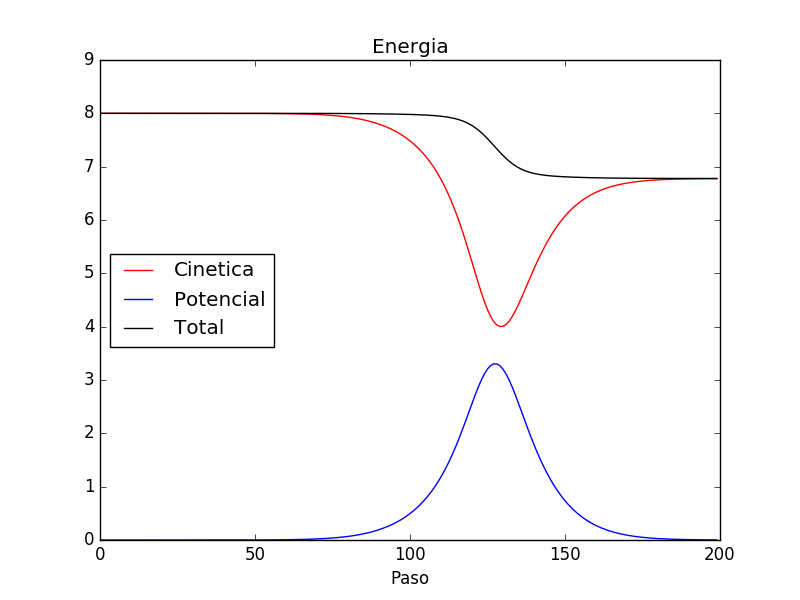
\includegraphics[trim = 20mm 0mm 15mm 10mm, clip, width=0.32\columnwidth]{energia_euler_0,01.png}}
	\subfigure[Runge-Kutta 2]{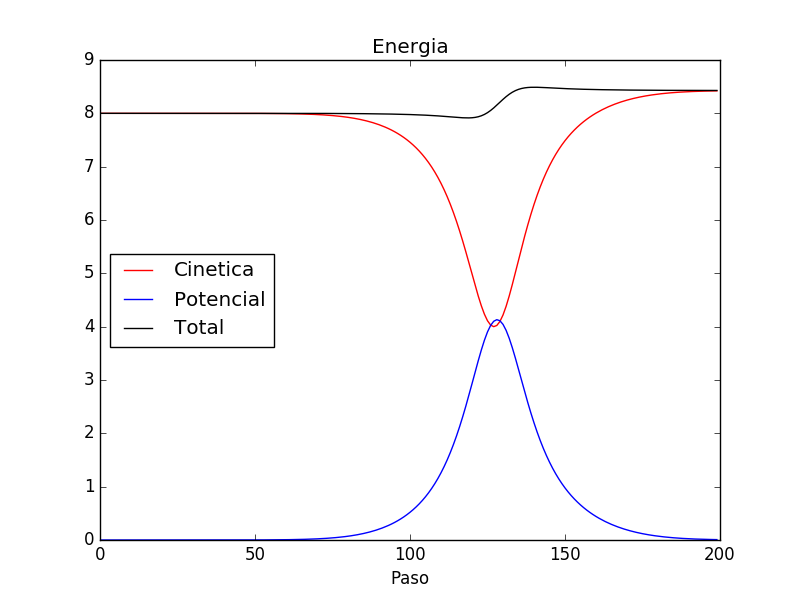
\includegraphics[trim = 20mm 0mm 15mm 10mm, clip, width=0.32\columnwidth]{energia_rk2_0,01.png}}
	\subfigure[Midpoint Rule]{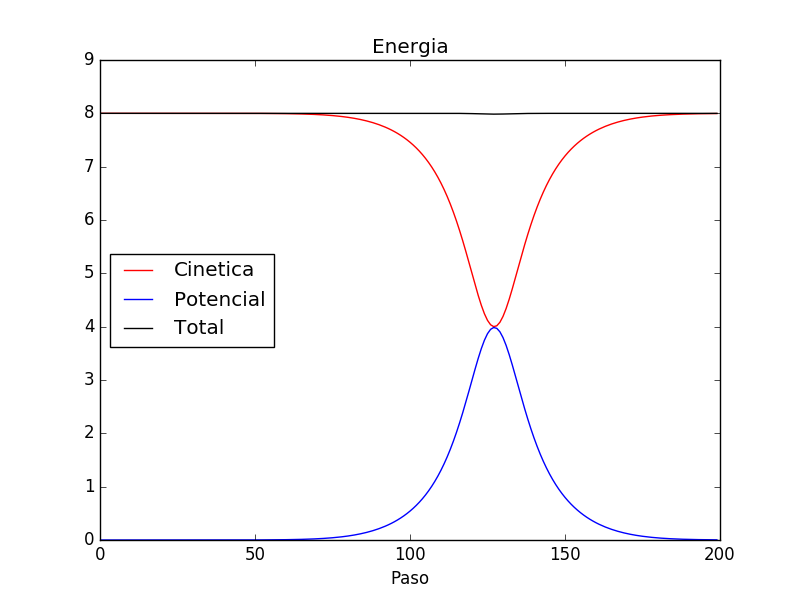
\includegraphics[trim = 20mm 0mm 15mm 10mm, clip, width=0.32\columnwidth]{energia_mpr_0,01.png}}
	\caption{Energía durante un choque para un potencial de Pauli con $D = 10000$ y $qo = 1 = po$. La trayectoria comenzó en el $(q, p) = (6, -4)$ y se integró con paso temporal $h=0.01$}
	\label{fig:energ_choq}
\end{figure}

Estos choques se realizaron para distintos valores de $h$ y se analizó la fluctuación relativa de energía (siempre positiva para el potencial de Pauli).
Los resultados pueden apreciarse en la \textbf{Figura \ref{fig:flucvsh}}, donde se confirma la clara superioridad de MPR a la hora de conservar la energía. 
Esto último resulta a priori esperable dado que MPR es un integrador simpléctico; no obstante, al ser resuelta la ecuación con un método de punto fijo, esto podía dejar de ser cierto.

\begin{figure}[h]
	\centering
	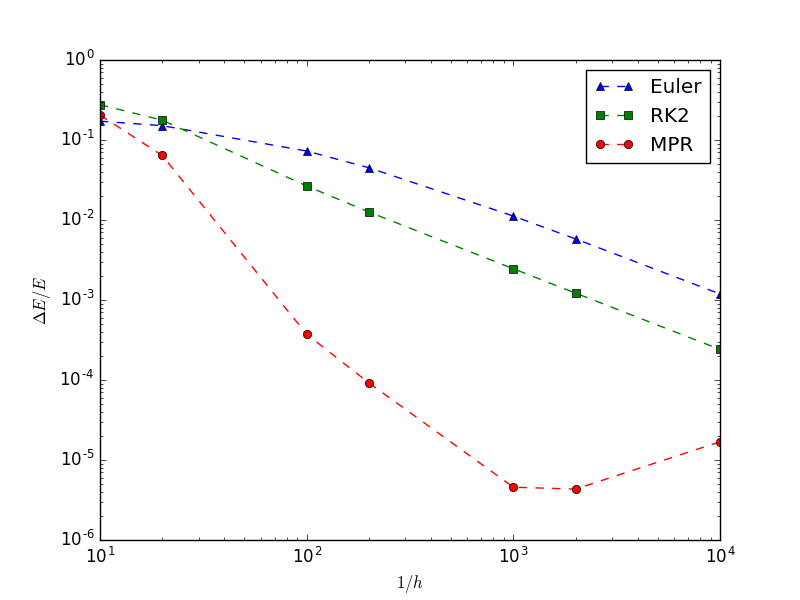
\includegraphics[trim = 0mm 0mm 15mm 10mm, clip, width=0.6\columnwidth]{fluct_vs_h.png}
	\caption{Fluctuaciones de energía en función de paso temporal para distintos integradores.}
	\label{fig:flucvsh}
\end{figure}

\subsection{Conservación del volumen de fases: Teorema de Liouville}

Otro criterio para calificar la efectividad de los integradores es la conservación del volumen de fases a lo largo de la evolución.
Para esto, realizamos una simulación tomando un conjunto de valores iniciales $(q_i, p_i)$ y evolucionándolos en paralelo.
En cada paso, asumiendo que cada punto era una elipse rígida de área definida, se calculó el volumen del conjunto de puntos como la suma de sus volumenes individuales.

Esto se hizo para curvas de rebote con 81 puntos en un cuadrado de $0.04\times0.04$ alrededor del $(6, 4)$ y los mismos parámetros de antes para Pauli.
Los resultados pueden apreciarse en la \textbf{Figura \ref{fig:vol_fas}}.

\begin{figure}[h]
	\centering
	\subfigure[h = 0.01]{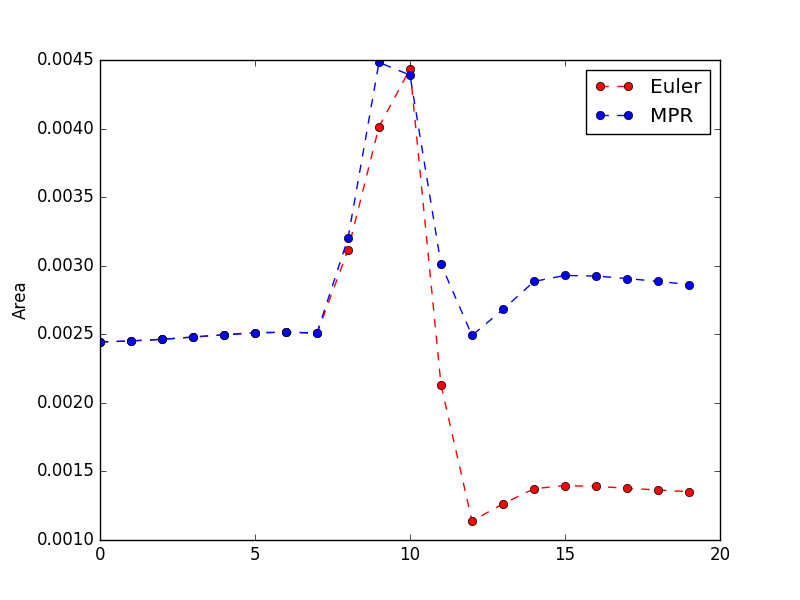
\includegraphics[trim = 20mm 0mm 15mm 10mm, clip, width=0.32\columnwidth]{vol_fas_0,01.png}}
	\subfigure[h = 0.005]{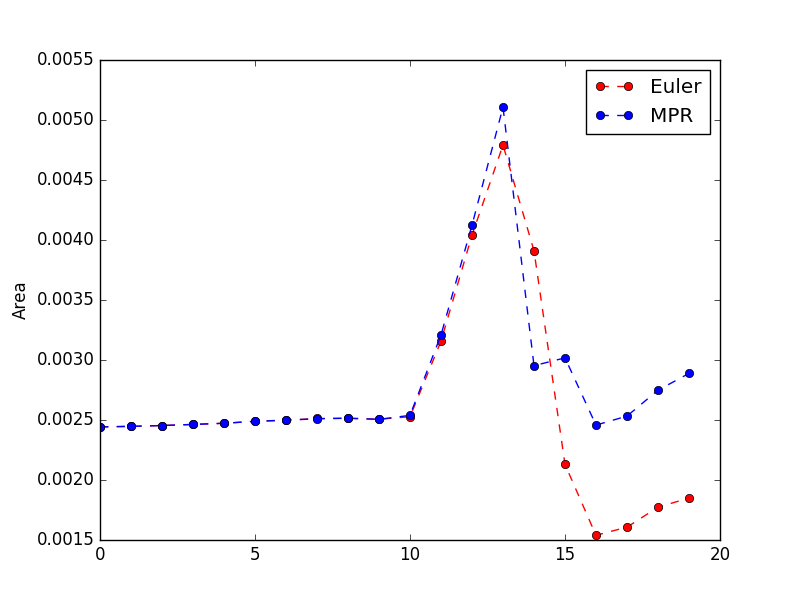
\includegraphics[trim = 20mm 0mm 15mm 10mm, clip, width=0.32\columnwidth]{vol_fas_0,005.png}}
	\subfigure[h = 0.001]{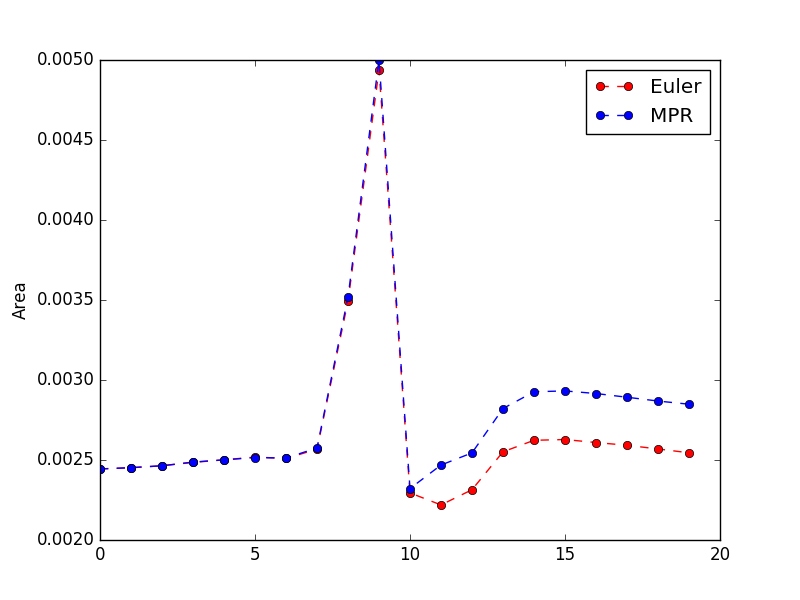
\includegraphics[trim = 20mm 0mm 15mm 10mm, clip, width=0.32\columnwidth]{vol_fas_0,001.png}}
	\caption{Volumen de un conjunto de puntos a lo largo de una curva de rebote. El pico corresponde al momento de máxima interacción.}
	\label{fig:vol_fas}
\end{figure}

Es importante aclarar que el pico de volumen se da en la región de la curva donde la interacción es máxima, momento en el cual los puntos tienden a alinearse en una curva 1D en lugar de un cuadrado.
Sin embargo, es importante que luego de ello los puntos vuelvan a su forma más cuadrada, lo cual se nota al ver que los volumenes recuperan su valor previo. 
Esto es un buen indicio y ocurre para $h=10^{-3}$ para ambos integradores, pero solo para el MPR en los otros 2 casos. 
En un tercer caso con $h=0.1$ que omitimos, ninguno de los 2 métodos cumplía esto.

Por lo tanto, vemos nuevamente que el integrador MPR tiene una mayor robustez, manteniendo las propiedades esperables para valores de $h$ mayores.


\section{Espacio de fases}

\subsection{Primeros resultados y propiedades generales}

Con el análisis anterior, concluimos elegir el integrador MPR para la evolución del sistema. 
Notando la dependencia de $H$ con $(q,p)$ según \eqref{eq:hamiltoneano}, buscamos las trayectorias en el espacio $(q,p)$.
Estas trayectorias cumplen que mantienen el valor de $H$ constante; son sus curvas de nivel. 

De forma análoga a lo anterior, las condiciones iniciales fueron con una partícula en el $(0,0)$ y la otra en un valor $(q_i, p_i)$. 
Luego, evolucionabamos el sistema muestreando los valores de $q = q_1 - q_2$, $p = p_1 - p_2$.
Así obteniamos una curva en el espacio de fases $(q,p)$; una curva de nivel de $H$.
Llamaremos a estas curvas definidas por la condición inicial $(q_i,p_i)$ como $C(q_i,p_i)$, tal que $H(C(q_i,p_i))=H(q_i, p_i)$.

Para muestrear por completo el espacio de fases, variamos el impulso inicial $p_i$ para $q_i$ constante y luego hicimos lo mismo para los estados iniciales $(-q_i,-p_i)$.
Un ejemplo de esto se encuentra en la \textbf{Figura \ref{fig:ej_fases}}, donde puede apreciarse la existencia de una \textit{región prohibida}; una región inaccesible para las curvas de nivel.

\begin{figure}[h]
	\centering
	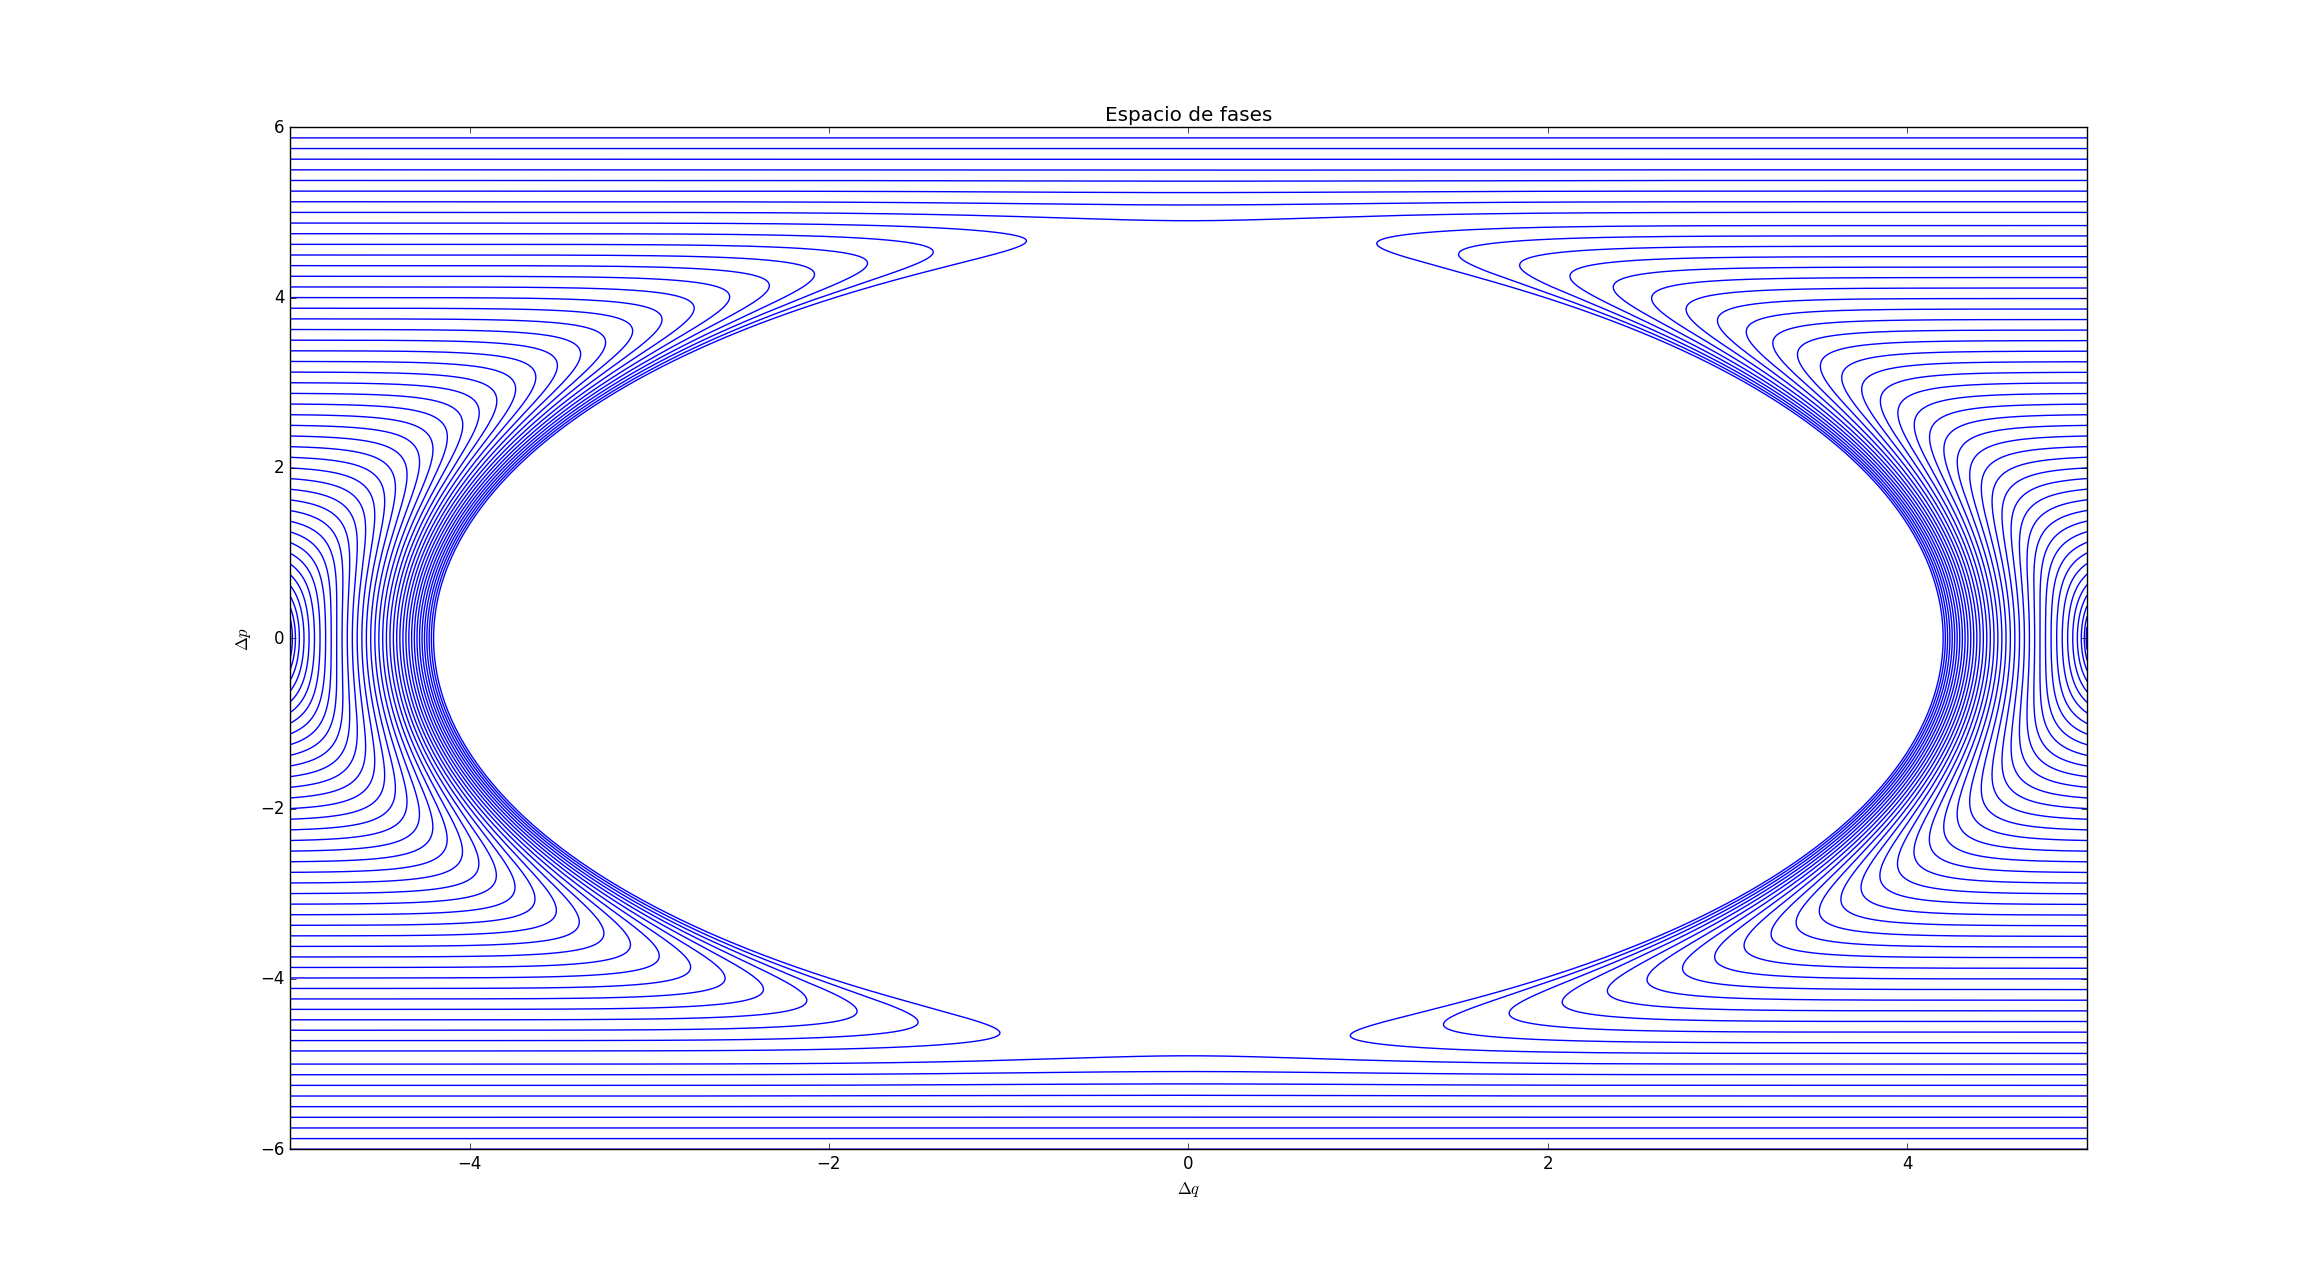
\includegraphics[trim = 0mm 0mm 15mm 10mm, clip, width=\columnwidth]{fases.png}
	\caption{Espacio de fases para $D=10^4$, $p_o=1=q_o=m$ y $h=10^{-3}$. Se evidencia una región inaccesible.}
	\label{fig:ej_fases}
\end{figure}

Es importante aclarar que debe tomarse $q_ip_i\leq 0$, de forma que las partículas efectivamente comiencen acercándose.
Además, a simple vista se aprecia la simetría que tiene el diagrama de fases frente a las reflecciones en el eje $q$ y $p$.
En particular, se cumple $C(q_i,p_i) = -C(-q_i,-p_i)$; se recorren en sentidos opuestos.  

Posteriormente, puede verse con claridad la diferencia entre los 2 regimenes del choque: rebote y atravesado.
El primer caso corresponde a curvas que no lográn alcanzar el $q=0$ y, por lo tanto, recorren el camino espejado (con impulso $-p$).
En su segmento más cercano al origen, resultan \textit{convexas} y definen justamente esta región inaccesible.
El segundo caso corresponde a trayectorias en las cuales las partículas logran superponerse ($q=0$) y luego continuan avanzando (se atraviesan).
En principio, estas curvas parecerían definir las cotas en $p$ de la región prohibida.

Sin embargo, veremos en breve que esto no es así, sino que la región prohibida queda univocamente definida por las curvas de rebote.
En particular, la transición de rebote a atraviese debe ser continua al ser el hamiltoneano suave.
Por lo tanto, las \textit{puntas} (donde $|q|$ es mínimo) de las curvas de rebote a izquierda y derecha deberian eventualmente tocarse para dar lugar a las curvas de atraviese.
De esta manera, existirá un par $(q_b, p_b)$ cuya curva de nivel tenga sus puntas tan cercanas a las de $(-q_b, -p_b)$ como se quiera.
Mediante una cuadratura sobre esta curva, es posible estimar el \textit{area de la región prohibida} $A$.

\subsection{Teorema $\Pi$}

Sin embargo, primero es necesario analizar los parámetros de los cuales dependerá este área $A$.
En principio las curvas $C$ solo pueden depender de los parámetros del hamiltoneano $q_o, p_o, m, D$. El valor de $P$ no puede afectar las curvas de nivel al ser constante.
Dado que el sistema tiene 3 unidades diferentes (masa, tiempo y distancia), el teorema $\Pi$ nos permitiría eliminar 3 de ellas, quedándonos con un único parámetro reducido.
Para esto, tomamos la expresión \eqref{eq:hamiltoneano} del hamiltoneano y redefinimos $q^* = q/q_o$, $p^* = p/p_o$, $H^* = Hm/p_o^2$.

\begin{equation}{\label{eq:ham_red}}
 H^*(q^*, p^*) = \frac{p^{*2}}{4} + \frac{Dm}{p_o^2}e^{-\frac{1}{2}(q^{*2}+p^{*2})} \equiv \frac{p^{*2}}{4} + D^* e^{-\frac{1}{2}(q^{*2}+p^{*2})}
\end{equation}

De esta forma, el parámetro $D^*$ resulta evidentemente el responsable de la forma del área prohibida. 
Como casos extremos, tenemos $D^* = 0$ con el hamiltoneano transformandose en el de partícula libre; las curvas de nivel son rectas horizontales y no existe región prohibida.
Para $D^* \rightarrow \infty$, el término cuadrático en $p^*$ resulta despreciable y las curvas de nivel serán círculos en el espacio $(q^*, p^*)$ (elipses en el espacio $(q,p)$).

En particular, dado que $A$ tiene unidades de posición por momento (area en el espacio $q,p$), el teorema $\Pi$ nos asegura que $A = q_op_o f(D^*) = q_op_o f(Dm/p_o^2)$.
Resulta interesante la clara asimetría entre los parametros $q_o$ y $p_o$; si $A$ depende de $D$, entonces no puede ser simétrica ante el intercambio $q_o \leftrightarrow p_o$.
Para que $A$ crezca con $D$ (esperable dado que regula la intensidad de la repulsión), debe ser $f'(x)\geq 0$.

Pero entonces, aunque $A$ resulta claramente creciente en $q_o$, no es obvio que crezca con $p_o$, lo cual arruinaría la noción de $p_o$ regulando las distancias de acercamiento en la dirección $p$.

\[ \dpart{A}{p_o} = q_o\left( f(Dm/p_o^2) - \frac{2Dm}{p_o^2}f'(Dm/p_o^2) \geq 0 \right) \]
\[ \Longleftrightarrow f(x) \geq 2x f'(x) \Longleftrightarrow  \int_1^t \frac{f'(x)}{f(x)}dx \leq \int_1^t\frac{1}{2x}dx \Longleftrightarrow \log{\left(\frac{f(x)}{f(1)}\right)} \leq \log{(\sqrt{x})} \]
\[ f(x) \leq f(1) \sqrt{x}\]

En resumen, tenemos 
\[A = q_op_of(D^*) \qquad \text{ con} \qquad f'(x)\geq 0 \text{ y } f(x)\leq f(1)\sqrt{x} \]


\subsection{Area prohibida}

Analizando la \textbf{Figura \ref{fig:ej_fases}}, pareceriamos estar en un caso $\alpha \gg 1$.
Por lo tanto, resultaría razonable muestrear el valor de área en función de $D^*$, esperando una transición suave a $A=0$ para $D^* \rightarrow 0$.
Para simular las unidades reducidas, resulta equivalente tomar $q_o = p_o = m = 1$ de forma que $D^* = D$; estaremos muestreando la función $f(x)$.

Con esto en mente, corremos simulaciones que muestreen las curvas $C$ para encontrar el mayor valor de $p_i$ tal que $C(q_i, p_i)$ para el cual tenemos un rebote para un $q_i=5q_o$ fijo.
Basicamente, estamos buscando el par $(q_b, p_b)$ que mencionamos previamente.
Esta búsqueda se hace en forma binaria, tomando un $p_{max}$ que cumpla que $C(q_i, p_{max})$ sea un atraviese, sabiendo que $C(q_i, 0)$ \textbf{\textit{siempre}} es un rebote. 
El $p_{max}$ se obtiene tomando un valor inicial $p_max = -3$ y duplicándolo hasta obtener un atraviese.
Con estos 2 valores de impulso, se itera la busqueda binaria hasta que $|p_{max}-p_{min}|\leq tol$, donde el valor de $tol$ dependía de $D$ según $tol \sim \sqrt{D}\times 10^{-4}$.
Esta tolerancia se tomó considerando que para $D=10^4$ una $tol = 10^{-2}$ resultaba apropiada y aprovechando que $A\leq \sqrt{D}$ por lo anterior.
El paso temporal se tomó como $h=10^{-3}$ para $D\leq 1000$, $h=5\times10^{-3}$ para $5000\leq D\leq 50000$ y $h=10^{-4}$ para $D\geq 100000$.

Los resultados pueden apreciarse en la \textbf{Figura \ref{fig:AvsD}} junto con algunos ejemplos del espacio de fases (con mayor definición cerca de la región de interés).
La primera observación es que $A=0$ para $D\leq 0.5$, donde las curvas de rebote son cóncavas para $q\approx 0$ a diferencia del caso $D\geq 0.5$ donde son convexas (como en el ejemplo 
de la \textbf{Figura \ref{fig:ej_fases}}). De hecho, puede apreciarse que para $D=0.5$, las curvas son prácticamente verticales, marcando el cambio de convexidad.

\begin{figure}[H]
	\centering
	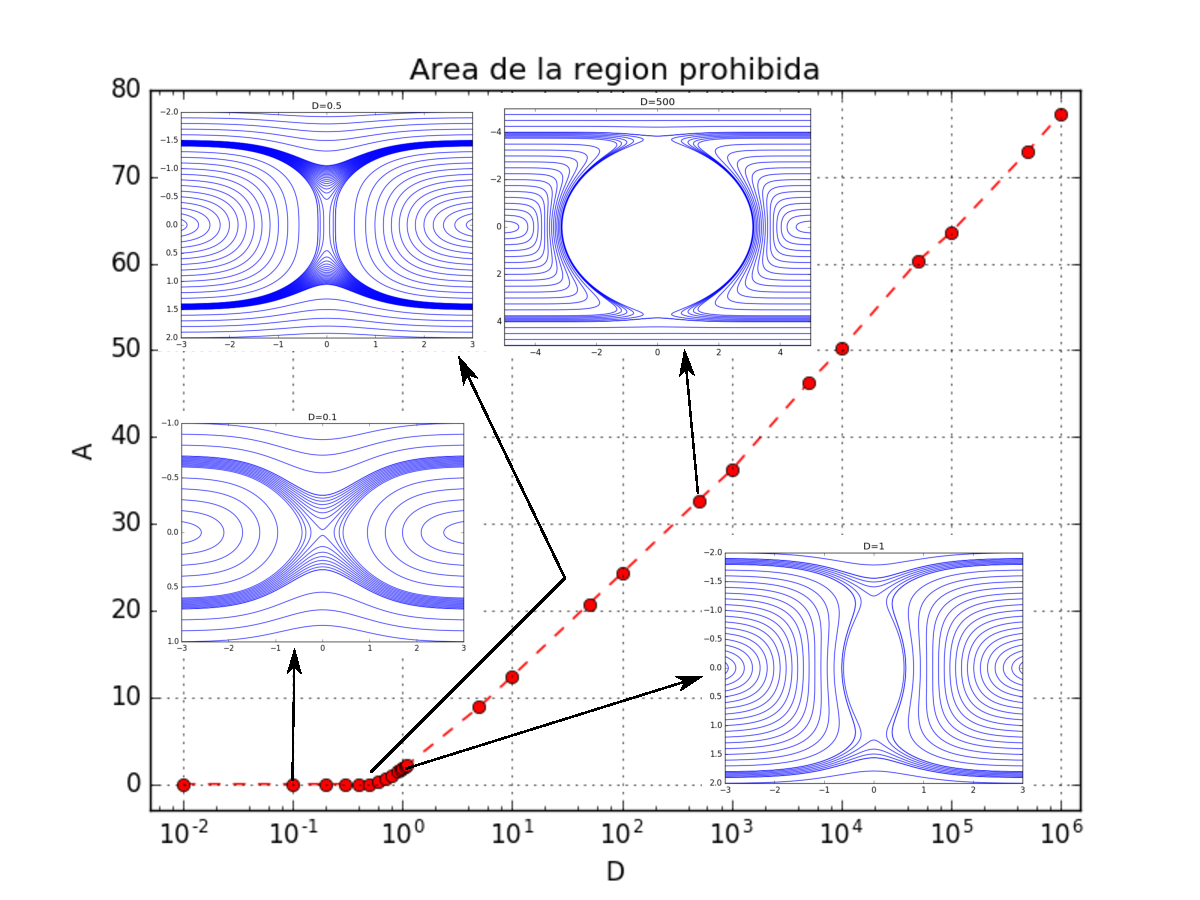
\includegraphics[trim = 0mm 0mm 15mm 10mm, clip, width=\columnwidth]{AvsD_full.pdf}
	\caption{Area prohibida en función de intensidad de potencial. Se muestran además algunos de los espacios de fase asociados. Se tiene $A=0$ para $D\leq 0.5$ y $A\sim \log{D}$ para $D\geq 1$.}
	\label{fig:AvsD}
\end{figure}

Para $D\geq 1$, tenemos $A \approx \alpha \log{D} + \beta$ con $\alpha = 10.88$ y $\beta = 1.174$.
Realmente, el ajusta $A(D)$ resulta más apropiado con un polinomio de grado 3 en $\log{D}$, pero esto no es relevante.
Lo relevante es confirmar que la cota $A(D) \leq A(1)\sqrt{D}$ se cumple apropiadamente y, por lo tanto, tenemos $\dpart{A}{p_o} \geq 0$.

Lo más sorprendente es, sin embargo, que $A$ se anule para $D\leq 0.5$. Esto puede obtenerse de forma analítica usando \eqref{eq:ham_red}.
Si la región prohibida no existe, entonces debe existir una curva de nivel $C$ arbitrariamente cerca del $(0,0)$. Entonces, expandiendo el hamiltoneano el Taylor

\[ H = \frac{p^2}{4} -\frac{D}{2}(p^2+q^2) = \frac{1}{2}\left[ p^2\left(\frac{1}{2}-D\right) - Dq^2 \right] \]

Para una curva de nivel $H\equiv E \geq 0$ pues el hamiltoneano es definido positivo y, por lo tanto

\[ 0\leq \frac{2E}{D} =  p^2\left(\frac{1-2D}{2D}\right) - q^2  \]

Si $1-2D\leq 0 $ tenemos una inconsistencia pues la suma de 2 numeros estrictamente negativos resulta positiva.
Tenemos una hiperbola como solución si y solo si $1-2D\geq 0 \Longrightarrow D \leq 0.5$. Por lo tanto, para $D \leq 0.5$ \textbf{no hay región prohibida} y por lo tanto debe ser $A=0$.
Por lo tanto, eliminamos la posibilidad de que el area $A$ fuese tan pequeña que no pueda medirse pero no nula.

\section{Conclusiones}

A pesar de la imposibilidad de encontrar un integrador simpléctico explícito, logramos implementar un integrador simpléctico explícito que resulta apropiado para integrar el problema de choque de 2 cuerpos.
Resolviendo de forma iterativa con un método de punto fijo, confirmamos que para 5 iteraciones el método ya lograba converger manteniendo las propiedades esperadas de un integrador simpléctico: conservación 
de energía y volumen de fases. 

Aunque todo lo anterior es muy importante, el método MPR tarda 5 veces lo que tarda Euler y 2.5 veces lo que tarda RK2 y Velocity Verlet (medido en evaluaciones de \texttt{fgorces}).
Esto podría ser un precio razonable a pagar por la simplecticidad, pero es ciertamente deseable achicar esto lo más posible; en especial considerando que para sistemas de muchas partículas es 
posible que sean necesarias aún más iteraciones. Esto aún está por verse.

Respecto al espacio de fases, resulta particularmente llamativa la inexistencia de una región prohibida para valores de $D \leq p_o^2/2m$, lo cual muestra que los parámetros del potencial deben elegirse
en función de esta variable reducida $D^* = Dm/p_o^2$. Conocido aproximadamente el comportamiento de $A(D^*)$ es posible buscar los parámetros que arrojen el valor de $A$ deseado; como por ejemplo $A\sim\hbar$.

Finalmente, pudimos ver que la forma más general del área prohibida es elíptica, alcanzando forma circular para valores de $D$ grandes. 
Esto no es un problema, dado que tomando los parámetros $p_o$ y $q_o$ adecuadamente, el área prohibida se reescala en $p$ y $q$. 
Así, podemos elegir los parámetros que nos den la relación de ejes de la elipse que nos parezca adecuada. 

\end{document}